% !TeX spellcheck = en_US
\chapter{Introduction}

Wind energy is widely becoming recognized as one of the most cost efficient renewable energy sources.
It is predicted that by the end of 2014 the worlds collected wind energy production will reach 360GW~\cite{worldwidewindcapacity}.
Heavyweight energy consumer USA has declared a goal of reaching 20\% wind energy of the total energy consumed in 2030~\cite{20percentenergy}, the European Union has committed to a similar goal of 20\% renewable energy by 2020~\cite{directive2009}.

Siemens Wind Power is one of the worlds leading producers of wind turbines, with a global market share of 9.5\% in 2012 \cite{worldmarketupdate2012}.
Siemens Wind Power is increasingly focusing on the offshore wind farm market.
The current setup of a wind farm requires additional infrastructure for management of the wind farm.
As well as the wind turbines the wind farm consists of a Wind Power Supervisor for operations that involve the entire farm and multiple High Performance Park Pilot, from here on refereed to as Park Pilots, for near realtime control of the turbines.
The Wind Power Supervisor and Park Pilots are centralised control points of the wind farm, having centralised control means that the system has single points of failure as well, which if it fails decreases the availability of the wind farm.
Furthermore the Wind Power Supervisor and Park Pilots does not scale automatically with the number of turbines, but needs hardware to be upgraded if too many turbines are added.

Since wind energy is recognized as one of the solutions to the renewable energy problem, wind farm size and capacity keeps increasing.
The need for scalability is thus not only a problem for Siemens Wind Power but for the entire industry.

The popularity of wind energy has lead to massive research within the area. The European Union has a number of sponsored projects among others:
\begin{itemize}
	\item INNWIND which focus is on accelerating the process of realising the 20MW turbine~\cite{INNWIND}.
	\item Aeolus which focus on the development of models that allows realtime predictions of wind flow~\cite{Aoelus}.
	\item EERA-DTOC which focus is on creating a software tool for optimizing offshore wind farm design and clusters of wind farms~\cite{eera-dtoc}.
\end{itemize}

Likewise USA has a number of projects most of them performed by Sandia National Laboratories or National Renewable Energy Laboratory. Projects that are interesting to this thesis is:
\begin{itemize}
	\item SWiFT which focus is on wake effects, turbine control and rotor development.
	\item Offshore Wind which focus on large rotor development and simulation algorithms.
	\item Active Power Control focus on using wind turbines for active control of the power grid
\end{itemize}

The area of decentralization in wind farm management and control has largely been neglected even though wind farms has reached a scale that is becoming increasingly hard to manage with a centralized approach.

\section{Siemens Wind Power case}

% Beskriv topologi
% Regulerings algoritmen tager kun 30 ms. 150 ms er cycle time

\label{sec:SiemensCase}
Siemens Wind Power builds wind farms of different sizes ranging from single turbines to well above one hundred turbines. \cite{simensOffShoreProjects, simensOnShoreProjects}.

Today turbines in a wind farm at Siemens are equipped with computers for the purpose of regulating power production parameters, data collection and for communication with the rest of the system. The current setup is illustrated on \cref{fig:currentSiemensSetup}. Every turbine is connected to a Wind Power Supervisor, which is a central component that aggregates data, perform calculations, store data and handle wind farm communication with the outside world. At Siemens up to eight Park pilots are present pr. wind farm and one Wind Power Supervisor.

For every transformer station there is a High Performance Park Pilot from here on refereed to as Park Pilot. The Park Pilots are responsible for park regulation. This is done by monitoring all the turbines performance parameters and issue correct set points for power production as illustrated on \cref{fig:dataComputationSequence}. Every turbine returns their current status to the Park Pilot, then the set points for each turbine is calculated in the Park Pilots and finally the new set points can be pushed to the turbines. 

Every turbine has a database for raw data logging purposes, this database is replicated to the Wind Power Supervisor.
The Wind Power Supervisor does data aggregation on data from each turbine as well as store a copy of the replicated data.
The turbines, Wind Power Supervisor and Park Pilots are connected with a gigabit network, which currently has plenty of extra capacity.
The system handles more than 50 control points and 200 measurement points and samples these every 50 ms.

\begin{figure}
	\centering
	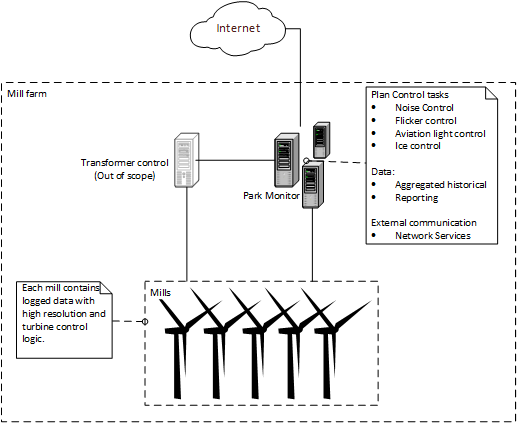
\includegraphics[width=0.7\textwidth,natwidth=610,natheight=642]{SystemOverviews.png} 
	\captionsetup{format=plain,font=footnotesize,labelfont={bf,defaultCapFont},labelsep=quad,singlelinecheck=no}
	\caption[The current Siemens wind farm system overview]{
		\label{fig:currentSiemensSetup} 
		\footnotesize{%
			The current Siemens wind farm system overview.
		}
	}
\end{figure}

\begin{figure}
	\centering
	\begin{sequencediagram} %Created using pgf-umlsd
		\newthread{reg}{:Park Pilot}
		\newinst[2]{turbine}{:Turbine}
	
		\begin{sdblock}{each turbine}{}
			\mess[1]{reg}{getCurrentStatus}{turbine}
			\mess[1]{turbine}{status}{reg}
		\end{sdblock}
		
		\begin{call}{reg}{calculateAllSetpoints()}{reg}{}
		\end{call}
	
		\begin{sdblock}{each turbine}{}
			\mess[1]{reg}{setNewSetpoint}{turbine}
		\end{sdblock}
					
	\end{sequencediagram}

	\captionsetup{format=plain,font=footnotesize,labelfont={bf,defaultCapFont},labelsep=quad,singlelinecheck=no}
	\caption[Regulator calculation sequence]{
		\label{fig:dataComputationSequence} 
		\footnotesize{%
			Regulator calculation sequence.
		}
	}
\end{figure}

\section{Thesis motivation}
\label{sec:ThesisMotivation}
Todays setup at Siemens Wind Power (\cref{sec:SiemensCase}) is an example of a system wished to be made less centralized. The current setup poses the following problems to Siemens:  

\begin{itemize} 
	\item Single point of failure. Should a Wind Power Supervisor or a Park Pilot fail, a part of the wind farm will become unavailable.
	\item Low scalability. The Wind Power Supervisors and Park Pilots does not scale with the number of turbines. This is reflected in the park regulation performance. Today a park regulation cycle-time is 150 ms. This cycle-time is set after worst case set point retrieval time, worst case new setpoint calculations and worst case time it takes to broadcast new setpoints. This ultimately depends on worst case number of turbines pr. Park Pilot.
\end{itemize}

Siemens wishes to decentralize the Wind Power Supervisor and Park Pilots by distributing their functionality to the turbines, utilizing the free capacity of the computers already residing in every turbine. This would increase availability by lowering the possibility of single point of failure. Furthermore this would increase scalability of the system, opening for performance optimizations of the park regulation cycle-time by detaching regulation performance from number of turbines pr. Park Pilot. 


\section{Problem statement}

The purpose of this thesis is to design, implement and evaluate a system solution for a Siemens windmill farm, where the Wind Park Supervisor and the Park Pilots are decentralized by utilizing the free capacity residing in every turbine for the Siemens Wind Power case. The solution must be able to provide the same features as the current solution. 

\paragraph{We present the following questions:}
\begin{itemize} 
	\item How can we best re-implement the current Siemens system (\cref{sec:SiemensCase}) as a system where the Wind Park Supervisor and the Park Pilots are decentralized?
	\item Can we, with the new decentralized solution, reduce the current regulation cycle time of 150 ms?
	\item Can we create a solution that scales so the number of turbines do not impact the regulation cycle time?
	\item Can we create a solution where removing one or more node from the system at runtime does not cause system failure?
\end{itemize}

The implementation of the system will be a prototype, which runs the developed solution, for proof of concept purposes. The prototype will be compared to the existing Siemens solution with respect to performance, availability and redundancy using an objective test metric we develop for the comparison.

%ASK SIEMENS HOW TO COMPARE AND MORE CONSTRAINTS??? 

%The purpose of this thesis is to design, implement and evaluate a distributed system solution for the Siemens Wind Power case. The solution must be able to provide the same features as the current solution. The goal of the new solution is to improve scalability, availability and performance by distributing the Park Pilot and the Wind Power Supervisor onto the turbines and thereby eliminate single point of failures and make performance scale with the amount of turbines within the wind farm. 

%To realize this the system must be redesigned as a distributed system. The solution must be able to handle external requests, communication between the nodes and distribution of data, according to the Siemens case. Furthermore the solution must have a single interface for control of, and interaction with, all the nodes, in order to maintain the illusion of the wind farm serving as a single system. This means ease of access must be maintained even though computation and data is distributed among nodes. Traffic must be routed to a turbine controllers with free capacity through a single interface, without external systems being aware of it.

%This roughly leaves three essential components: A component that handles distribution of data, a component that handles communication between nodes and a load balancer, to keep track of available resources on each node. The aim to investigate, analyze and evaluate state of the art technologies within each component area and choose the technologies best suited for the Siemens case. The technologies will be weighed in terms of features with regards to the Siemens case and performance.
%
%Furthermore we aim to develop a prototype, which runs the developed solution, for proof of concept purposes. The prototype will be compared to the existing Siemens solution with respect to performance, availability and redundancy. ASK SIEMENS HOW TO COMPARE AND MORE CONSTRAINTS??? 
%
%The Siemens case presents the following constraints to the project:
%\begin{itemize}
%	\item CPU power. Our solution must be able to run on a standard consumer hardware.
%	\item Network bandwidth. Siemens uses gigabit network.
%	\item Topology. Siemens wind farms uses ring and star topology.
%\end{itemize}



% % The below snippet might come handy later on % % %
% % % % % % % % % % % % % % % % % % % % % % % % % % %
%A distributed system is a network of hardware or software components, which communicates and coordinate their actions only by message passing\cite{coulouris2005distributed}, as illustrated on \cref{fig:distributedSystem}. Each component have their own local memory every component and interact with each other in order to achieve a common goal. The nodes can be physically close, connected via a local network, or geographically distant, connected by a wide area network. An important goal of a distributed system is location transparency\cite{coulouris2005distributed} to create the illusion of the entire system acting as a single computer even though it is comprised of several nodes. Examples of distributed systems vary from aircraft control systems to the Internet to massively multiplayer online games. 
% Er det bare mig eller er det lidt rigeligt at sige at systemet agere som en enkelt computer? Lad hellere sige noget om at opnå et fælles mål? Multiplayer spil er vel ikke distribuerede systemer, men mere server client systemer.

%\begin{figure}
%	\centering
%	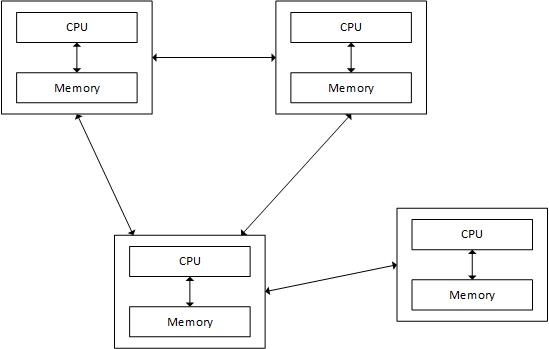
\includegraphics[width=0.7\textwidth,natwidth=510,natheight=542]{DistributedSystem.jpg} 
%	\captionsetup{format=plain,font=footnotesize,labelfont={bf,defaultCapFont},labelsep=quad,singlelinecheck=no}
%	\caption[Distributed Computing System with 2 nodes]{
%		\label{fig:distributedSystem} 
%		\footnotesize{%
%			A distributed system with 4 nodes.
%		}
%	}
%\end{figure}

%Distributed systems offer many benefits over centralized systems including the following\cite{IBM2005TXSeries}:
%\begin{itemize}
%	\item Scalability: It is easy to add nodes to the system, should the size of the system increase.
%	\item Redundancy: Several nodes can provide the same service, so if a node crashes, there are many to replace it. Additionally, from a cost perspective, each node does not have to be expensive, because many smaller nodes can be used as replacement.
%\end{itemize}
% Vi burde nok også snakke om ulemper? Og det er vel bare ting som er mulige at opnå?

